\subsection{Tabelle}
\label{subsec:table}
Die Tabelle ist einer der meist genutzten Datenstrukturen um Daten zu repräsentieren. Aus diesem
Grund wurde die Tabelle in der Analyse mit aufgenommen. Dabei wurde eine Tabelle von
\emph{N} Elementen generiert und die Ergebnisse der Messungen im folgenden Diagram zusammengetragen:

\begin{figure}[h]
    \centering
    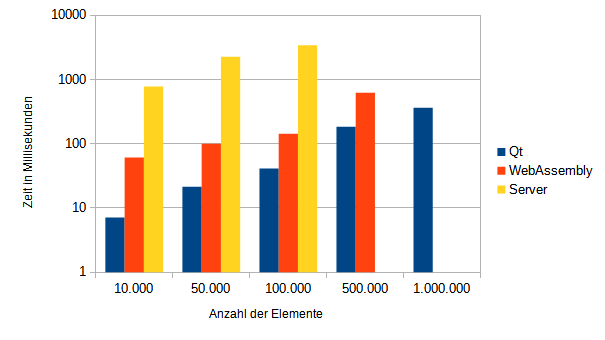
\includegraphics[width=\textwidth, center]{Analyse/Tabelle}
    \caption[Ergebnisse der Messungen von der Erzeugung einer Tabelle in Millisekunden]{Ergebnisse
    der Messungen von der Erzeugung einer Tabelle in Millisekunden}
    \label{img:table}
\end{figure}

Interessant ist zu erkennen, dass die Server-Architektur bei 500.000 Elementen in einem
\emph{Timeout} resultierte. Dieses Vehalten lässt sich dadurch erklären, da die Elemete vom
Server zum Client übertragen werden müssen.

Die WebAssembly-Architektur wiederum, resultierte erst bei 1.000.000 Elementen in einem
\emph{Timeout}. Hier mussten die Elemente nicht zuerst vom Server zum Client übertragen werden,
sondern standen direkt zum Verarbeiten auf dem Client zur Verfügung. Der \emph{Timeout} bei 1.000
.000 Elementen, lässt sich dadurch erklären, dass der \emph{Rendering-Prozess} bei vielen
Elementen zu lange dauert.